%!TEX root = ../main.tex
\doublespacing
\chapter{Observations of Radio Scattering in the Solar Corona compared to Computational Modelling.}
\label{chap:observations_vs_theory}
As was discussed previously, the anisotropic diffusion treatment of radio wave scattering predicts certain source characteristics for a radio burst at locations from the solar disk, assuming the unscattered burst is a point source. To date, this has not been compared qualitatively to observations of Type III radio bursts. In this chapter I utilise the direct visibility fitting method described in Chapter \ref{chap:measuring_source_sizes} and apply it to hundreds of type III radio bursts. I showcase the difference between these observations and computational modelling and discuss possible causes for the discrepancy.

\section{Introduction}
\label{sec:obsvtheory_intro}
\cite{Kontar2019} perform Monte Carlo ray-tracing simulations of radio waves in a spherically symmetric solar corona. They assume an anisotropic distribution of density fluctuations with a relative r.m.s value of $\varepsilon = 0.8$ and varying levels of anisotropy $\alpha$. They start their model as a point source emitting at $\omega = 1.1 \omega_p(R_s)$ for a source at radial distance $R_s$ emitting fundamental plasma emission. They use the PARKER1960\cite{Parker1960} model (approxmiated by 3 power laws for computational simplicity) for a spherically symmetric corona wiht constant temperature and other constants chosen to agree with observation.	
THere investigation lead them to the conclusion the anisotropy will cause the apparant source size to change as a function of postion from the disk centre. Strong anisotropy $\alpha = 0.3$ has a large effect on source size whereas weak anisotropy $\alpha = 0.5$ does not show much of a trend.

\section{Method}
\label{sec:obsvtheory_method}
By fitting their interferometric visibilities as described in Chapter \ref{chap:measuring_source_sizes}, the size and position of 30 Type III radio bursts over the period of 04 April 2019 to 14 April 2019 were found. The bursts were identified in LOFAR beamformed observations and their peak time determined using an automatic peak finding algorithm. Figure \ref{fig:dynamic_spectrum_070419} shows the automatically identified bursts at 30 MHz. In total, 320 bursts were identified in this way. Unfortunately, due to the strength of these bursts, the calibration of interferometric data failed for $\sim 90 \%$ of them. 30 bursts were identified manually as having successfully been calibrated and their properties fit. As well as determining the source shape and position at its peak, the area of the source over its duration was also measured. This was done by fitting a straight line to the source area over the duration of the burst, which was estimated to be 1 second before its peak and 2 seconds afterwards.

\begin{figure}
\centering
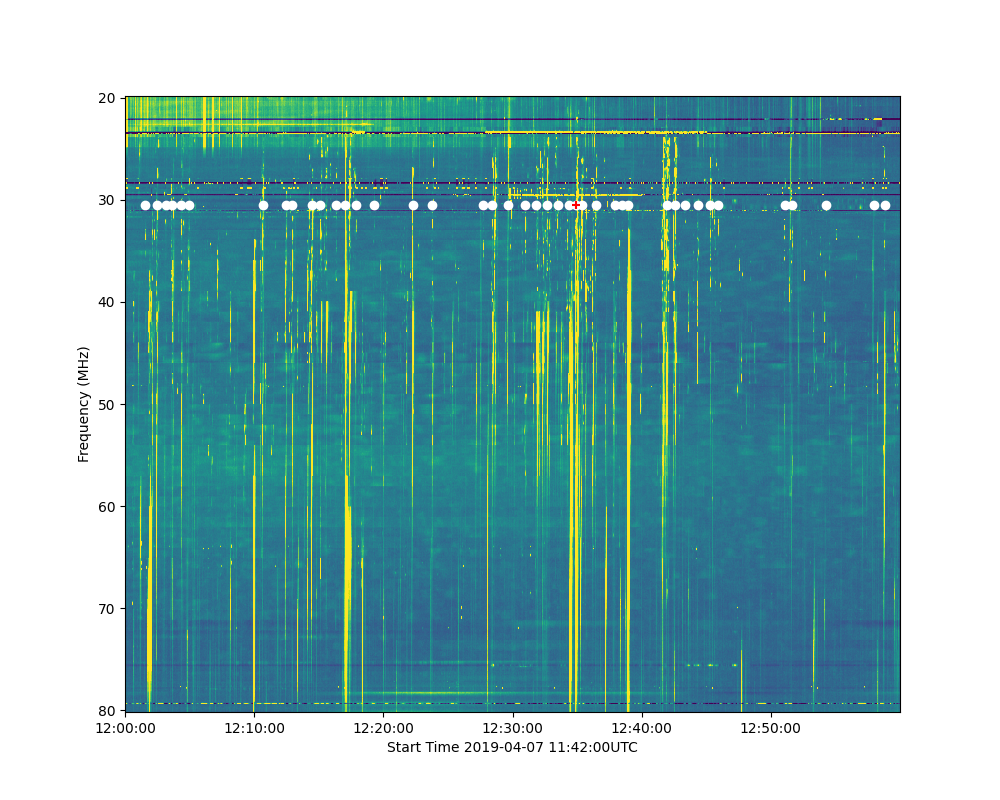
\includegraphics[width=\columnwidth]{peak_times_30MHz_2019-04-07T120000_130000.png}
\caption[Dynamic spectrum of Type III storm on 07 April 2019.]{Dynamic spectrum of Type III storm on 07 April 2019. The white dots indicate the bursts identified by an automatic peak finding algorithm, the red cross indicates the brightest burst.}
\label{fig:dynamic_spectrum_070419}
\end{figure}

\section{Results}
\label{sec:obsvtheory_results}
Each fitted type III burst is overlayed on a synoptic AIA 193\AA  map in Figure \ref{fig:synoptic_bursts}. It is clear from the figure that most burst share a similar size and ``aspect ratio", which I define as the ratio of the fwhm in the minor direction to that in the major, despite their relatively widespread origin in relation to the Sun's disk.

\begin{figure}
\centering
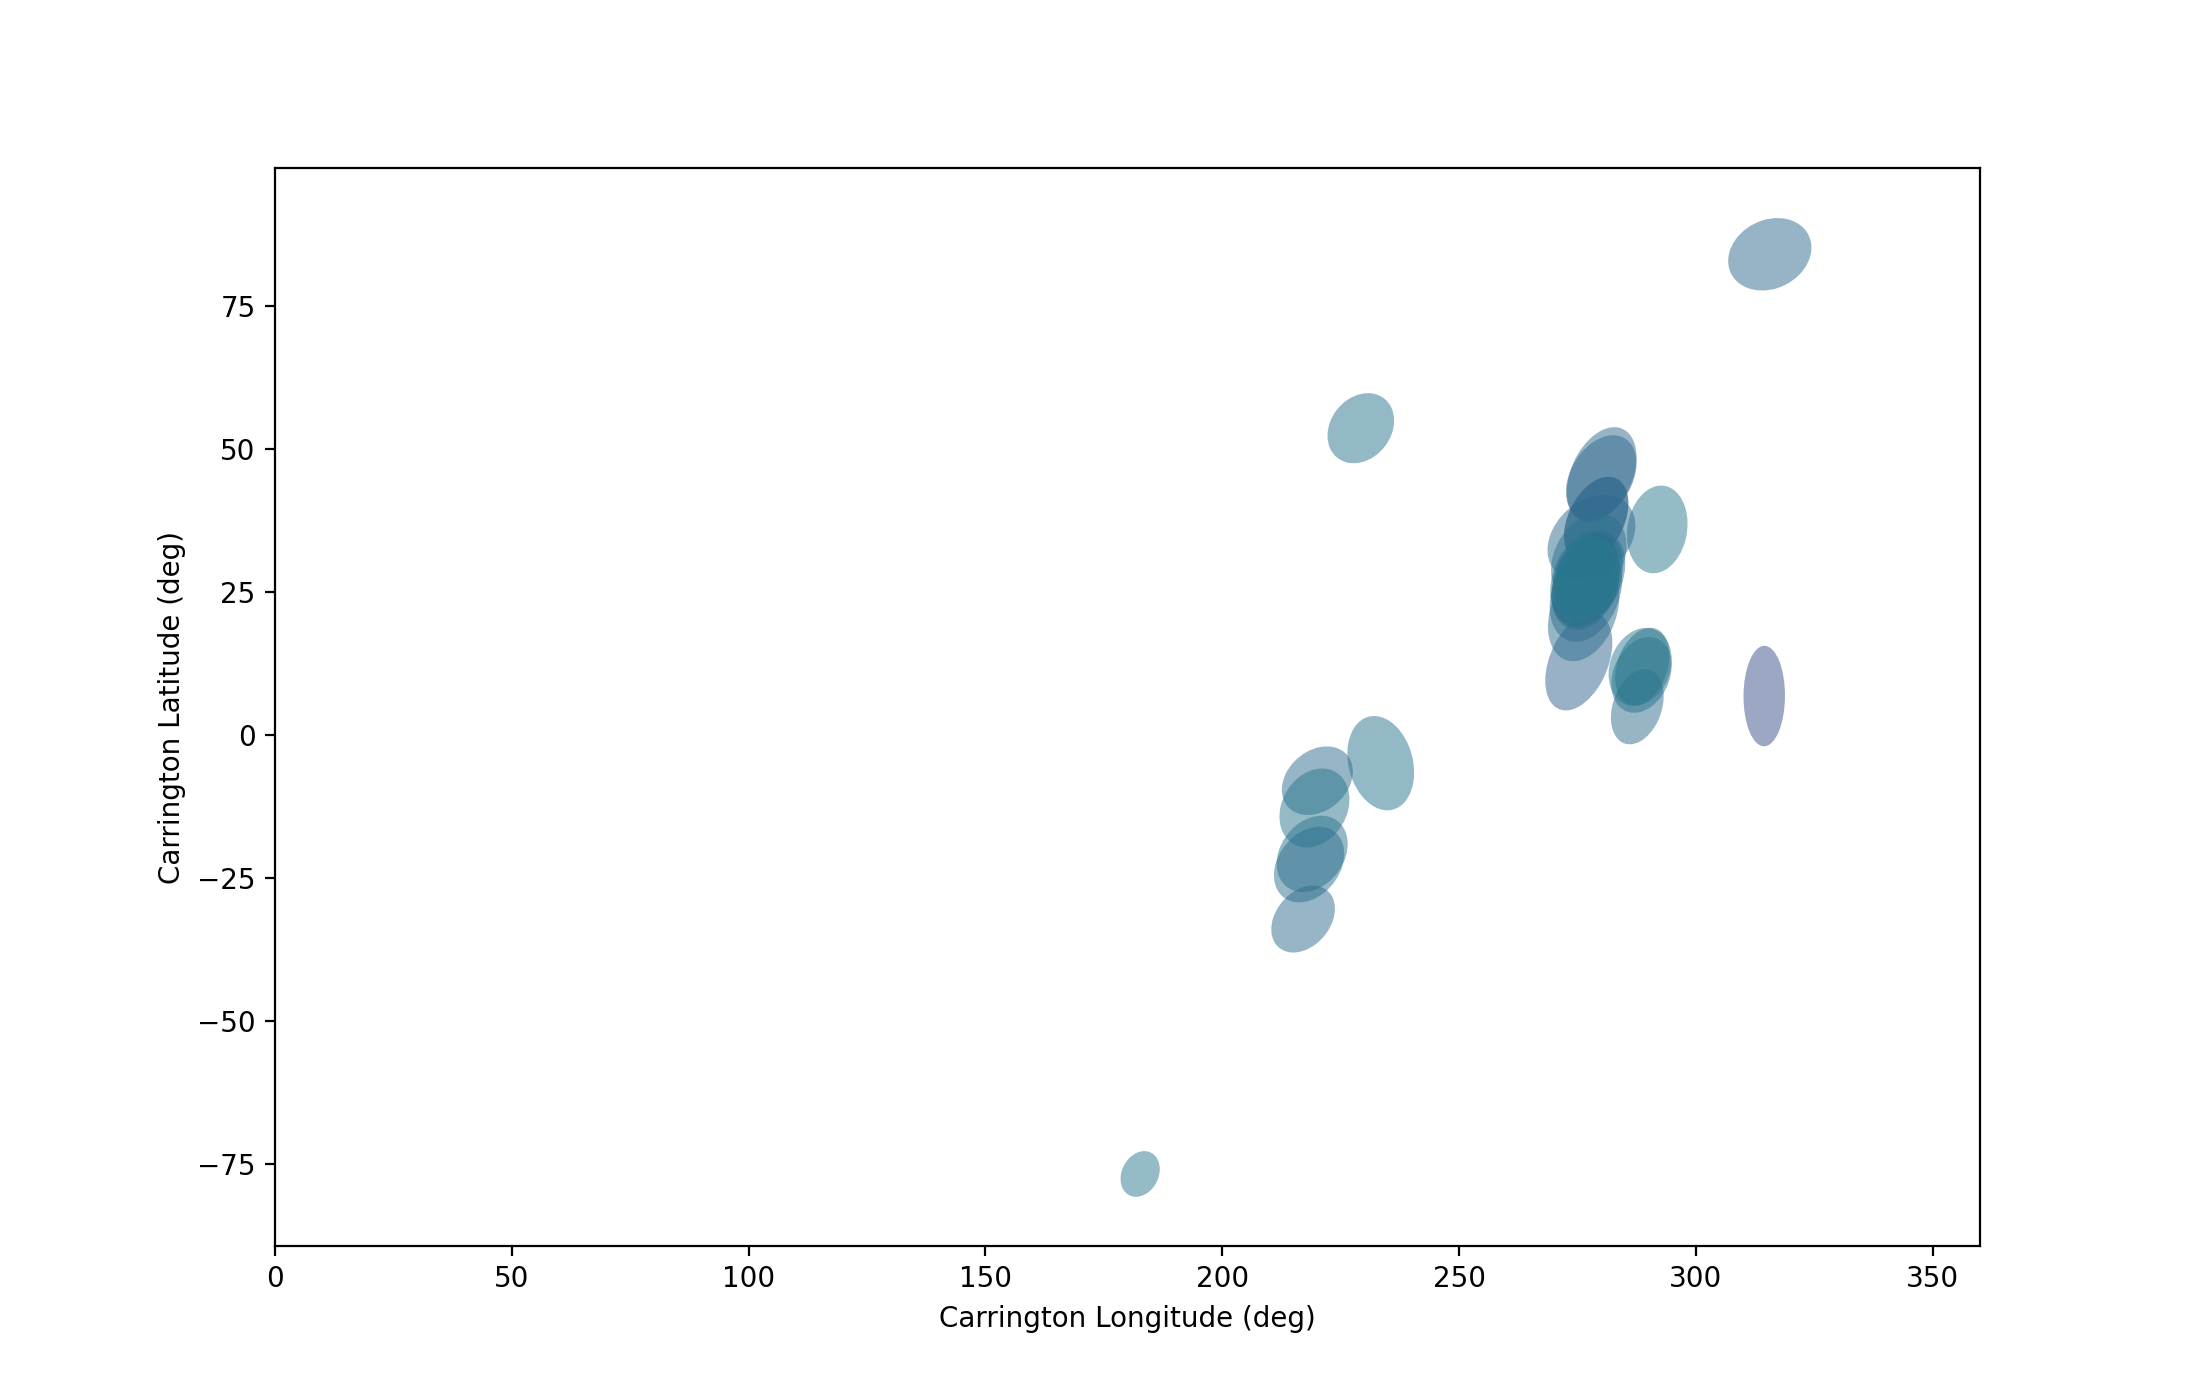
\includegraphics[width=\columnwidth]{burst_ellipses_carrington.png}
\caption[Synoptic AIA 193\AA  map overlayed with Type III radio bursts.]{A 193 \AA  AIA synoptic map where each fitted radio burst is overplotted. }
\label{fig:synoptic_bursts}
\end{figure}

The size of each burst, here denoted by the full width half maximum in the major and minor direction, is plotted against the distance from the disk centre in the x and y direction in Figure \ref{fig:fwhm_comp}. There is no obvious trend towards bigger/smaller bursts with increasing distance from disk centre and, most strikingly, in direct contrast to the prediction by \cite{Kontar2019} there is no trend in the ``aspect ratio" of the bursts, which is expected to trend towards 1 near disk centre and $< 1$ near the limb. The mean size of the bursts $\sim 16$ arcmin and $\sim 11$ arcmin in the major and minor directions respectively. This is consistent with previous work at these frequencies \citep{Kontar2017, Murphy2021}.

\begin{figure}
\centering
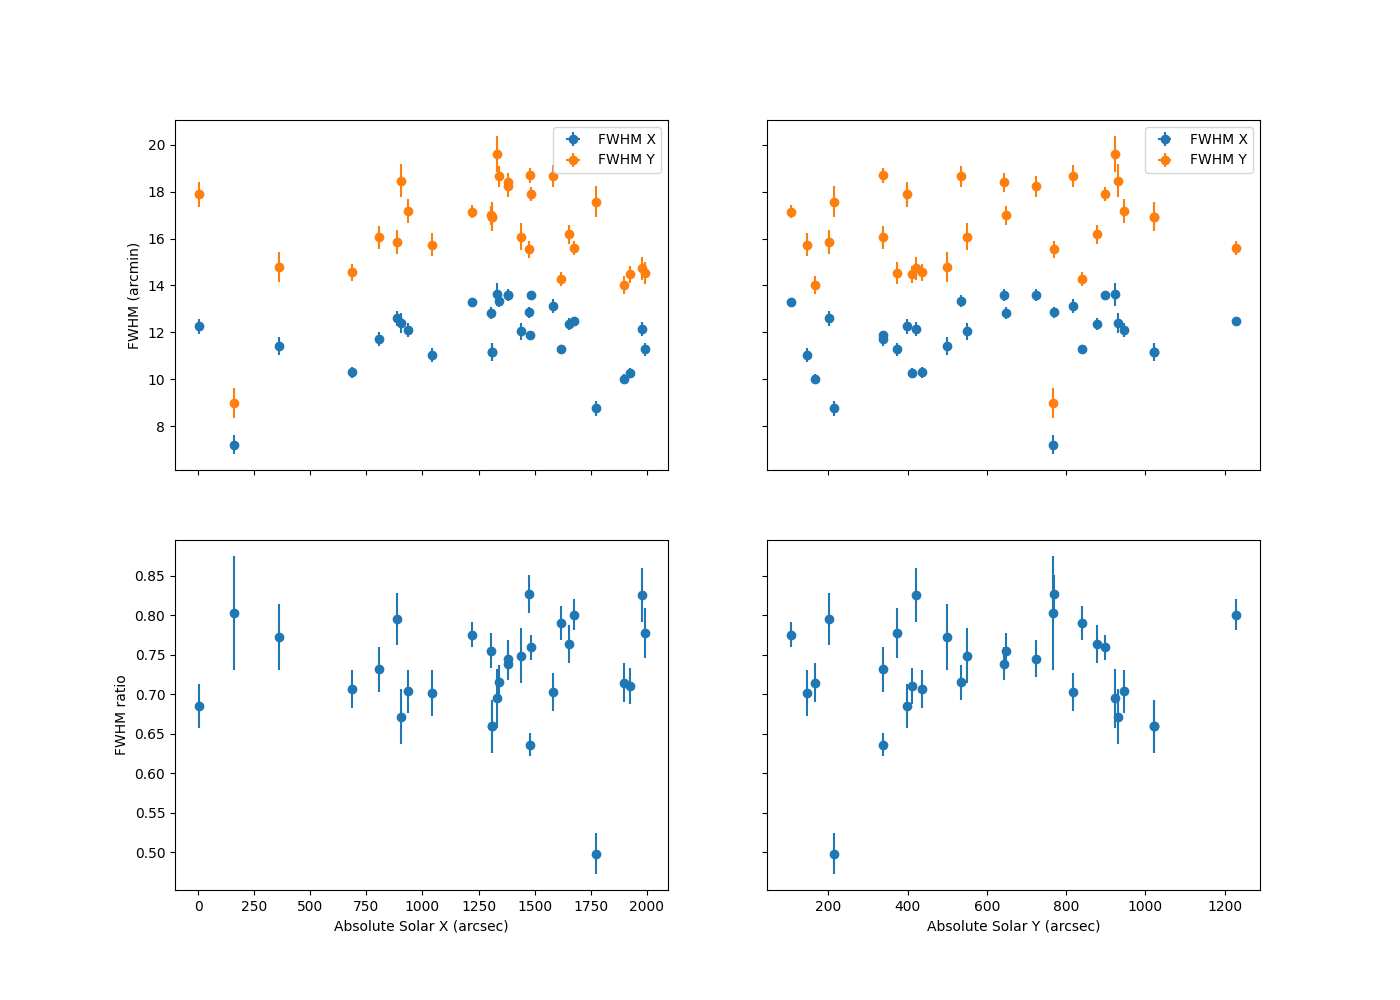
\includegraphics[width=\columnwidth]{fwhm_comparison.png}
\caption[Directly fitted Type III burst sizes as a function of position relative to disk centre.]{A comparison of the directly fitted Type III burst sizes and their location relative to the disk centre in the x and y direction. Top row, FWHM in x (blue) and y (orange) as a function of their distance from the disk centre in the x (left) and y (right) direction. Bottom row, same as above except showing the ``aspect ratio" of each burst.}
\label{fig:fwhm_comp}
\end{figure}

\section{Discussion}
\label{sec:obsvtheory_discussion}
The results given here are largely consistent with models of scattering through anisotropic density fluctuations in a spherically symmetric corona apart from one major sticking point. No trend towards more circular source sizes is evident in this data which suggests one of a number of things: The whole model of anisotropic scattering is wrong, it's inapporpriate to consider a spherically symmetric corona, the anisotropy is not constant, Type III bursts are not point sources and have inherent size. 

